\section{Boundary conditions}
\textbf{Start program}
To start the program you must be on a computer with the program on it. Then you just have to run the file. If you want the program to have the full functionality at synchronize the calendar, you must have a network connection. 
\newline
\newline
\textbf{Shutdown program}
To shut down the program you must be in the program, and be able to click on the lock down button. 
We have also clarified some boundary use cases that we have put in our use case diagram, to handle some different boundary exceptions. 
\newline
\newline
\textbf{Offline Mode}
Offline mode is a state the system goes in, when it cannot connect to the internet. It limits the system to save changes locally. 

\textbf{Failures}
\begin{itemize}
	\item \textbf{ShareFail:} Extends NetworkFail. If the network fails, the calendar and events cannot be shared. The system will then go offline, and try sharing again, when a connection is established. 
	\item \textbf{SyncFail:} Extends NetworkFail. If the network fails, the calendar and events cannot be synchronized and saved in the Database. The system will go offline, and save data locally, and try to sync, when a connection is established.
	\item \textbf{DBConnectionFail:} Is extended by the Server. The system has a working network connection but the system cannot connect to the Server. 
\end{itemize}
The handling of most persistent objects is already described in the use cases during analysis, and in the access control matrix (figure \ref{fig:AccessControlMatrix}) 
Hence we identify new boundary use cases. We have included six new use cases to our use case diagram with is represented in the RAD (section 3.4.2). 


\begin{figure}[h]
\centering
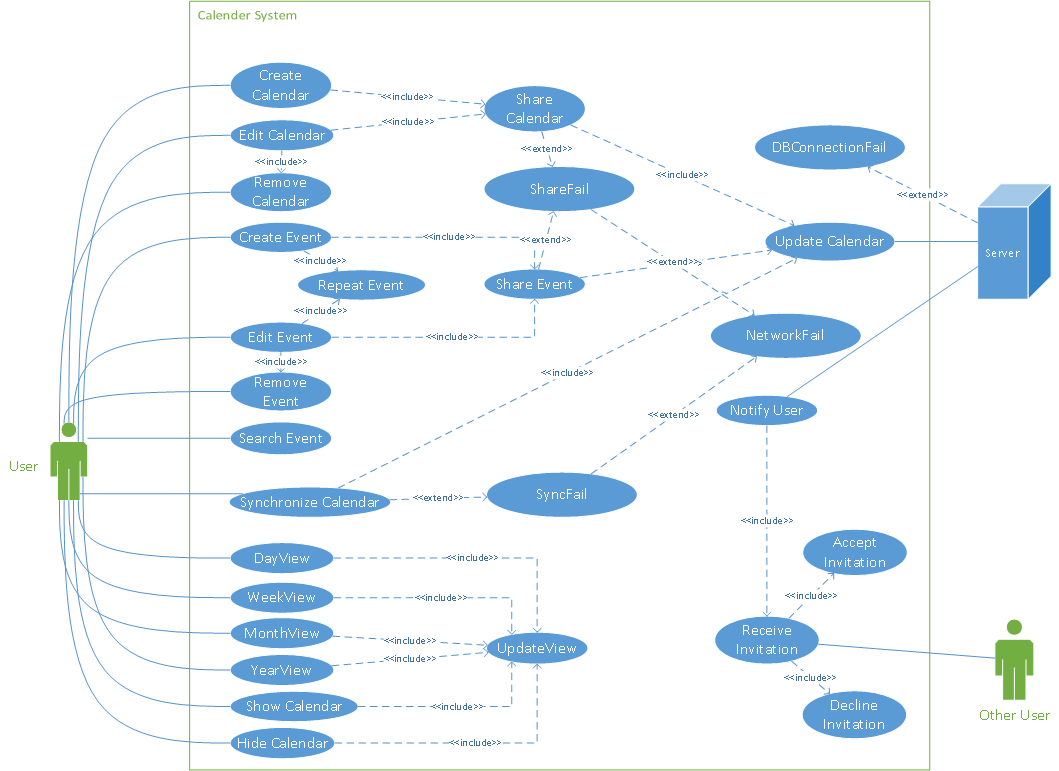
\includegraphics[width=160mm]{UMLUseCaseDiagram.png}
\caption{Updated UML Use Case diagram with  boundary conditions \label{overflow}}
\label{figur:usecase}
\end{figure}